\chapter{Redoxevenwichten en de vergelijking van Nernst}\label{ch:b1:nernst}

Zet een zinkstrip in een oplossing van zinksulfaat en een koperstrip in
een oplossing van koper(II)\-sulfaat, verbind de twee oplossingen met een
buis vol zoutoplossing en de twee metalen met een draad via een led: de
led brandt. De reactie van zink met koperionen, die in één bekerglas
alleen de oplossing opwarmt, stuwt nu elektronen door een draad. Een
batterij is deze opstelling, verpakt; een pH-meter en een
chloride-elektrode zijn haar meetende neven. Dit hoofdstuk maakt de
uitwisseling van elektronen kwantitatief: \omterm{def:b1:nernst:oxidation-number}{oxidatiegetallen} om de
elektronen te tellen, \omterm{def:b1:nernst:electrode-potential}{elektrodepotentialen} om de koppels te rangschikken,
en de \omterm{thm:b1:nernst:nernst}{vergelijking van Nernst} om ze als functie van de concentratie te
volgen.

\begin{recall}
Het schoolboek (jaar 11 en 12) definieerde \omterm{def:b1:nernst:couple}{oxidatoren} en \omterm{def:b1:nernst:couple}{reductoren},
schreef \omterm{def:b1:nernst:couple}{halfreacties} op, bouwde cellen uit twee metalen en twee
oplossingen, en las de zink-kopercel als een batterij. Het
\omterm{def:b1:extent-q-and-k:quotient}{reactiequotiënt} en de evenwichtsconstante zijn die van
\cref{ch:b1:extent-q-and-k}; de \omterm{def:b1:extent-q-and-k:activity}{activiteiten} zijn $c/c^\circ$ voor
opgeloste stoffen en $p/p^\circ$ voor gassen, 1 voor zuivere vaste
stoffen en vloeistoffen.
\end{recall}

\section{Oxidatiegetallen en koppels}

\begin{definition}[Oxidator, reductor, redoxkoppel, halfreactie]\label{def:b1:nernst:couple}
Een \emph{oxidator}\index{oxidator} is een deeltje dat elektronen kan
opnemen, een \emph{reductor}\index{reductor} een deeltje dat ze kan
afstaan. Een oxidator Ox en de reductor Red die hij wordt, vormen een
\emph{redoxkoppel}\index{redoxkoppel} Ox/Red, beschreven door zijn
\emph{halfreactie}\index{halfreactie}
$\alpha\,\mathrm{Ox} + n\,\mathrm{e^-} \rightleftharpoons
\beta\,\mathrm{Red}$, kloppend gemaakt in atomen met \ce{H2O} en \ce{H+}
waar nodig, en in lading met de elektronen.
\end{definition}

Een redoxreactie is de uitwisseling van elektronen tussen twee koppels:
de \omterm{def:b1:nernst:couple}{oxidator} van het ene wordt gereduceerd terwijl de \omterm{def:b1:nernst:couple}{reductor} van het
andere geoxideerd wordt, en de elektronen vallen tegen elkaar weg. Om ze
in een ingewikkeld deeltje te tellen, krijgt elk atoom een
\omterm{def:b1:nernst:oxidation-number}{oxidatiegetal}.

\begin{definition}[Oxidatiegetal]\label{def:b1:nernst:oxidation-number}
Het \emph{oxidatiegetal}\index{oxidatiegetal} van een atoom in een
deeltje is de lading die het zou dragen als elke binding verbroken werd
door beide bindingselektronen aan het meest elektronegatieve atoom te
geven (gelijk verdeeld tussen twee identieke atomen). Het wordt in
Romeinse cijfers geschreven: ijzer(III), \ce{Mn^{+VII}} in het
permanganaation.
\end{definition}

\begin{proposition}[Regels voor oxidatiegetallen]\label{prop:b1:nernst:on-rules}
\begin{enumerate}
  \item Een atoom in een element heeft \omterm{def:b1:nernst:oxidation-number}{oxidatiegetal} 0; een eenatomig ion
        heeft zijn lading.
  \item De \omterm{def:b1:nernst:oxidation-number}{oxidatiegetallen} van de atomen van een deeltje tellen op tot
        zijn lading.
  \item Waterstof is $+$I (behalve in metaalhydriden, $-$I); zuurstof is
        $-$II (behalve in peroxiden, $-$I, en gebonden aan fluor); fluor is
        $-$I.
  \item In een \omterm{def:b1:nernst:couple}{halfreactie} is het aantal elektronen gelijk aan de
        verandering van het \omterm{def:b1:nernst:oxidation-number}{oxidatiegetal} van het element dat verandert,
        maal het aantal atomen ervan.
\end{enumerate}
\end{proposition}

\begin{proof}
1 en 2: het verbreken van alle bindingen behoudt de lading, en tussen
identieke atomen wordt niets overgedragen. 3: waterstof is minder
elektronegatief dan elk niet-metaal waaraan het bindt
(\cref{ch:b1:periodicity}) en meer dan de alkalimetalen; zuurstof is
elektronegatiever dan elk element behalve fluor, en in \ce{O-O} wordt het
gedeelde paar verdeeld. 4: H en O behouden hun getallen, zodat de enige
atomen waarvan de fictieve lading verandert die van het betrokken element
zijn, en de elektronen verschijnen in de \omterm{def:b1:nernst:couple}{halfreactie} precies om die
ladingsverandering te compenseren.
\end{proof}

\begin{method}[Oxidatiegetallen van een deeltje]\label{met:b1:nernst:oxidation-numbers}
Geef H, O, F en de ionen hun gebruikelijke getallen; het getal van het
overblijvende atoom volgt uit regel 2. In \ce{MnO4-}: $x + 4(-2) = -1$,
$x = +7$. In \ce{Cr2O7^2-}: $2x - 14 = -2$, $x = +6$. In \ce{S4O6^2-} is
het gemiddelde $+2.5$; de \omterm{def:b1:lewis-resonance-vsepr:lewis}{lewisstructuur} toont twee soorten zwavel.
\end{method}

\begin{method}[Een halfreactie kloppend maken]\label{met:b1:nernst:balance-by-on}
\begin{enumerate}
  \item Maak het element kloppend dat van \omterm{def:b1:nernst:oxidation-number}{oxidatiegetal} verandert.
  \item Voeg de elektronen toe: de verandering van het \omterm{def:b1:nernst:oxidation-number}{oxidatiegetal} maal
        het aantal atomen.
  \item Maak de lading kloppend met \ce{H+} (zure oplossing) of \ce{OH-}
        (basische oplossing).
  \item Maak waterstof en zuurstof kloppend met \ce{H2O}; controleer
        zuurstof als laatste.
\end{enumerate}
Voor het permanganaation in zuur milieu: Mn gaat van $+$VII naar $+$II,
dus 5 elektronen; de lading links is $-1 - 5 = -6$ en rechts $+2$, dus
$8\,\ce{H+}$; daarna $4\,\ce{H2O}$:
\ce{MnO4- + 8H+ + 5e- -> Mn^2+ + 4H2O}.
\end{method}

\section{Elektrochemische cellen}

\begin{definition}[Elektrochemische cel]\label{def:b1:nernst:cell}
Een \emph{elektrochemische cel}\index{elektrochemische cel} bestaat uit
twee \emph{halfcellen}\index{halfcel}, elk gevormd door een koppel en een
elektronische geleider, de elektrode, verbonden door een ionische
geleider, vaak een \emph{zoutbrug}\index{zoutbrug} (een gel of buis met
een geconcentreerd inert zout zoals kaliumnitraat). De elektrode waar
oxidatie plaatsvindt, is de \emph{anode}\index{anode}, die waar reductie
plaatsvindt de \emph{kathode}\index{kathode}. De
\emph{celspanning}\index{celspanning} is het verschil in elektrische
potentiaal tussen de twee elektroden, positieve pool min negatieve pool,
gemeten wanneer er geen stroom loopt.
\end{definition}

\begin{omfigure}
\begin{tikzpicture}[font=\small, >={Stealth}]
  \pic at (0,0) {beaker={0.7}{omDef!14}};
  \pic at (3.6,0) {beaker={0.7}{omDef!32}};
  \pic at (-0.3,0.25) {electrode={black!35}};
  \pic at (3.9,0.25) {electrode={orange!70!brown}};
  \pic at (0.35,0.55) {saltbridge={2.9}};
  \pic (m) at (1.8,4.3) {meter={V}};
  \draw[thick] (-0.15,2.65) |- (m-a);
  \draw[thick] (4.05,2.65) |- (m-b);
  \node[anchor=east] at (-0.95,1.0) {\ce{Zn}};
  \node[anchor=west] at (4.45,1.0) {\ce{Cu}};
  \node at (0.25,-0.35) {\ce{Zn^2+}, \ce{SO4^2-}};
  \node at (3.6,-0.35) {\ce{Cu^2+}, \ce{SO4^2-}};
  \draw[->, omProp, thick] (-0.15,3.35) -- (0.8,3.35) node[above, midway] {$\mathrm{e^-}$};
  \draw[->, omProp, thick] (2.8,3.35) -- (3.75,3.35) node[above, midway] {$\mathrm{e^-}$};
  \node[anchor=east] at (-0.9,2.3) {$-$ anode};
  \node[anchor=west] at (4.6,2.3) {kathode $+$};
  \node[font=\scriptsize, align=center] at (1.8,2.75) {zoutbrug\\ \ce{K+} $\rightarrow$ \quad $\leftarrow$ \ce{NO3-}};
  \node[font=\scriptsize] at (-0.1,-0.8) {\ce{Zn -> Zn^2+ + 2e-}};
  \node[font=\scriptsize] at (3.7,-0.8) {\ce{Cu^2+ + 2e- -> Cu}};
\end{tikzpicture}

{\small De zink-kopercel (daniellcel). Zink wordt geoxideerd aan de \omterm{def:b1:nernst:cell}{anode},
de negatieve pool; koperionen worden gereduceerd aan de \omterm{def:b1:nernst:cell}{kathode}, de
positieve pool. De elektronen stromen door de uitwendige keten van zink
naar koper; in de \omterm{def:b1:nernst:cell}{zoutbrug} bewegen de kationen naar de \omterm{def:b1:nernst:cell}{kathode} en de
anionen naar de \omterm{def:b1:nernst:cell}{anode}, zodat elke oplossing neutraal blijft.}
\end{omfigure}

Een cel wordt als één regel geschreven, de \omterm{def:b1:nernst:cell}{anode} links: \ce{Zn} $|$
\ce{Zn^2+} $\|$ \ce{Cu^2+} $|$ \ce{Cu}, met enkele strepen voor de
grensvlakken en een dubbele streep voor de \omterm{def:b1:nernst:cell}{zoutbrug}. Met alle
concentraties op \qty{1}{mol/L} is de spanning ervan \qty{1.10}{V}. De
reactie die verloopt wanneer de cel stroom levert,
\ce{Zn + Cu^2+ -> Zn^2+ + Cu}, is dezelfde die in één bekerglas zou
plaatsvinden; door de \omterm{def:b1:nernst:cell}{halfcellen} te scheiden worden de elektronen door de
draad gedwongen, waar ze arbeid kunnen verrichten.

\section{Elektrodepotentialen}

Een spanning is een verschil: alleen verschillen tussen twee \omterm{def:b1:nernst:cell}{halfcellen}
kunnen gemeten worden. Daarom wordt eens en voor altijd een
referentiehalfcel gekozen.

\begin{definition}[Elektrodepotentiaal, standaardpotentiaal]\label{def:b1:nernst:electrode-potential}
De \emph{standaardwaterstofelektrode}\index{standaardwaterstofelektrode}
is een platina-elektrode in contact met waterstofgas onder
\qty{1}{bar} en een ideale oplossing van \ce{H+} met \omterm{def:b1:extent-q-and-k:activity}{activiteit} 1. De
\emph{elektrodepotentiaal}\index{elektrodepotentiaal} $E$ van een \omterm{def:b1:nernst:cell}{halfcel}
is de spanning van de cel die gevormd wordt met de
standaardwaterstofelektrode links:
$E = V_{\text{halfcel}} - V_{\text{SWE}}$. Wanneer elk deeltje van het
koppel \omterm{def:b1:extent-q-and-k:activity}{activiteit} 1 heeft, is het de
\emph{standaardpotentiaal}\index{standaardpotentiaal}
$E^\circ$ van het koppel, een constante bij een gegeven temperatuur.
\end{definition}

\begin{omfigure}
\begin{tikzpicture}[font=\small, >={Stealth}]
  \pic at (0,0) {beaker={0.72}{omDef!14}};
  % glass jacket, open at the bottom, with the gas inlet on the right
  \draw[om glass] (-0.32,0.35) -- (-0.32,3.0) -- (0.32,3.0) -- (0.32,2.55)
    -- (0.95,2.55) (0.32,2.35) -- (0.95,2.35) (0.32,2.35) -- (0.32,0.35);
  \draw[thick] (0,0.9) -- (0,3.45);
  \fill[black!60] (-0.16,0.5) rectangle (0.16,0.9);
  \foreach \x/\y in {0.45/0.45, 0.55/0.75, 0.48/1.05, -0.45/0.5, -0.52/0.85}
    \draw[omDef!70] (\x,\y) circle (0.055);
  \draw[->] (1.9,2.45) node[right] {\ce{H2}, \qty{1}{bar}} -- (1.0,2.45);
  \draw (0.12,0.7) -- (1.5,0.2) node[right] {geplatineerd platina};
  \draw (-0.6,1.1) -- (-1.4,1.6) node[left] {\ce{H+}, activiteit 1};
  \node[anchor=west] at (0.05,3.45) {naar de stroomkring};
\end{tikzpicture}

{\small De \omterm{def:b1:nernst:electrode-potential}{standaardwaterstofelektrode}: waterstofgas borrelt over een
platinaplaatje dat bedekt is met fijn platina, gedompeld in een oplossing
waarin \ce{H+} \omterm{def:b1:extent-q-and-k:activity}{activiteit} 1 heeft. Haar koppel is \ce{H+}/\ce{H2}, met
afspraakgewijs potentiaal 0.}
\end{omfigure}

De waterstofelektrode is onhandig in gebruik; laboratoria meten tegen een
handiger \omterm{def:b1:nernst:cell}{halfcel} waarvan de potentiaal bekend is.

\begin{definition}[Referentie-elektrode]\label{def:b1:nernst:reference-electrode}
Een \emph{referentie-elektrode}\index{referentie-elektrode} is een \omterm{def:b1:nernst:cell}{halfcel}
waarvan de potentiaal vastligt en bekend is: de zilver-zilverchloride-elektrode
(een zilverdraad bedekt met zilverchloride in een chloride-oplossing met
vaste concentratie) of de kalomelelektrode (kwik in contact met
\ce{Hg2Cl2} en een chloride-oplossing).
\end{definition}

De tabel hieronder geeft de \omterm{def:b1:nernst:electrode-potential}{standaardpotentialen} die in dit deel
gebruikt worden; de verticale schaal van de volgende paragraaf toont de
gangbaarste.

\begin{omfigure}
\begin{tabular}{lr@{\qquad}lr}
\hline
koppel & $E^\circ$ (V) & koppel & $E^\circ$ (V) \\
\hline
\ce{Li+}/\ce{Li} & $-3.04$ & \ce{Cu^2+}/\ce{Cu} & 0.34 \\
\ce{K+}/\ce{K} & $-2.94$ & $[\ce{Fe(CN)6}]^{3-}$/$[\ce{Fe(CN)6}]^{4-}$ & 0.36 \\
\ce{Na+}/\ce{Na} & $-2.71$ & \ce{Cu+}/\ce{Cu} & 0.52 \\
\ce{Mg^2+}/\ce{Mg} & $-2.36$ & \ce{I2}/\ce{I-} & 0.53 \\
\ce{Al^3+}/\ce{Al} & $-1.68$ & \ce{O2}/\ce{H2O2} & 0.69 \\
\ce{Zn^2+}/\ce{Zn} & $-0.76$ & \ce{Fe^3+}/\ce{Fe^2+} & 0.77 \\
\ce{Fe^2+}/\ce{Fe} & $-0.41$ & \ce{Hg2^2+}/\ce{Hg} & 0.80 \\
\ce{Ni^2+}/\ce{Ni} & $-0.24$ & \ce{Ag+}/\ce{Ag} & 0.80 \\
\ce{Pb^2+}/\ce{Pb} & $-0.13$ & \ce{Br2}/\ce{Br-} & 1.08 \\
\ce{H+}/\ce{H2} & 0 & \ce{O2}/\ce{H2O} & 1.23 \\
\ce{S4O6^2-}/\ce{S2O3^2-} & 0.02 & \ce{MnO2}/\ce{Mn^2+} & 1.23 \\
\ce{Cu^2+}/\ce{Cu+} & 0.16 & \ce{Cl2}/\ce{Cl-} & 1.36 \\
\ce{AgCl}/\ce{Ag} & 0.22 & \ce{PbO2}/\ce{Pb^2+} & 1.46 \\
\ce{Hg2Cl2}/\ce{Hg} & 0.27 & \ce{MnO4-}/\ce{Mn^2+} & 1.51 \\
 & & \ce{HClO}/\ce{Cl2} & 1.63 \\
 & & \ce{H2O2}/\ce{H2O} & 1.76 \\
\hline
\end{tabular}

\smallskip
{\small \omterm{def:b1:nernst:electrode-potential}{Standaardpotentialen} bij \qty{25}{\celsius}, berekend uit de
getabelleerde standaardvormingsenergieën van Gibbs van de deeltjes van
elk koppel. Ze kunnen enkele honderdsten volt afwijken van andere
compilaties.}
% ledger: dfg:Li+_ao, dfg:K+_ao, dfg:Na+_ao, dfg:Mg2+_ao, dfg:Al3+_ao, dfg:Zn2+_ao, dfg:Fe2+_ao, dfg:Ni2+_ao, dfg:Pb2+_ao (computed in figdata/bachelor-1/standard-potentials.py)
% ledger: dfg:S4O62-_ao, dfg:S2O32-_ao, dfg:Cu2+_ao, dfg:Cu+_ao, dfg:AgCl_cr, dfg:Cl-_ao, dfg:Hg2Cl2_cr, dfg:Fe_CN63-_ao, dfg:Fe_CN64-_ao, dfg:I-_ao (same script)
% ledger: dfg:H2O2_ao, dfg:Fe3+_ao, dfg:Hg22+_ao, dfg:Ag+_ao, dfg:Br-_ao, dfg:H2O_l, dfg:MnO2_cr, dfg:Mn2+_ao, dfg:PbO2_cr, dfg:MnO4-_ao, dfg:HClO_ao (same script)
\end{omfigure}


\section{De vergelijking van Nernst}

\begin{theorem}[Vergelijking van Nernst]\label{thm:b1:nernst:nernst}
Voor een koppel $\alpha\,\mathrm{Ox} + n\,\mathrm{e^-} \rightleftharpoons
\beta\,\mathrm{Red}$, met eventueel andere deeltjes (\ce{H+}, \ce{H2O},
\ce{Cl-}) aan een van beide kanten, wordt de \omterm{def:b1:nernst:electrode-potential}{elektrodepotentiaal} gegeven
door de \emph{vergelijking van Nernst}\index{vergelijking van Nernst}
\[
  E = E^\circ + \frac{RT}{nF}\ln\frac{\prod a_{\text{ox-kant}}^{\nu}}{\prod
  a_{\text{red-kant}}^{\nu}}
  = E^\circ + \frac{0.059}{n}\log\frac{a(\mathrm{Ox})^\alpha\,\cdots}{a(\mathrm{Red})^\beta\,\cdots}
  \quad\text{bij \qty{25}{\celsius}},
\]
waarin elke \omterm{def:b1:extent-q-and-k:activity}{activiteit} haar \omterm{def:b1:extent-q-and-k:extent}{stoichiometrisch getal} draagt en de factor
$RT\ln 10/F = \qty{0.059}{V}$ bij \qty{298}{K}.
\end{theorem}

\admitted{De \omterm{thm:b1:nernst:nernst}{vergelijking van Nernst} volgt uit het verband tussen de
gibbsenergie van een reactie en de spanning van de cel, dat in het deel
van jaar~2 wordt afgeleid.}

\begin{example}[Drie koppels]\label{ex:b1:nernst:examples}
\ce{Cu^2+}/\ce{Cu}: $E = 0.34 + 0.030\log[\ce{Cu^2+}]$ (metallisch koper
heeft \omterm{def:b1:extent-q-and-k:activity}{activiteit} 1).
\ce{Fe^3+}/\ce{Fe^2+}: $E = 0.77 + 0.059\log([\ce{Fe^3+}]/[\ce{Fe^2+}])$.
\ce{MnO4-}/\ce{Mn^2+}: $E = 1.51 + \frac{0.059}{5}\log
\frac{[\ce{MnO4-}][\ce{H+}]^8}{[\ce{Mn^2+}]}$; bij gelijke concentraties
permanganaat en mangaan(II) is $E = 1.51 - 0.094\,\mathrm{pH}$: het
oxiderend vermogen van permanganaat daalt naarmate de pH stijgt.
\end{example}

Een tienvoudige verandering van een concentratie verschuift de
potentiaal met $0.059/n$ volt: enkele tientallen millivolt. Daarom is een
spanning die tot op de millivolt gemeten wordt een nauwkeurige maat voor
een concentratie, het principe van de pH-elektrode en van de
chloride-elektrode van het weekendprobleem.

\begin{history}[Walther Nernst]
\begin{minipage}[t]{0.22\linewidth}\vspace{0pt}
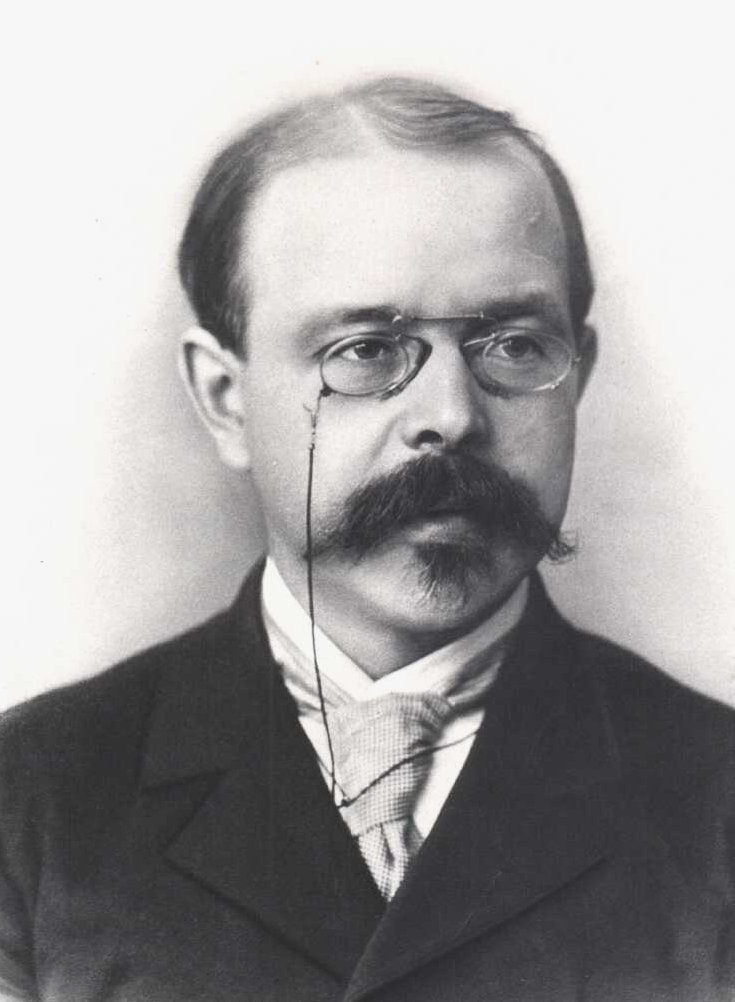
\includegraphics[width=\linewidth]{images/book2/nernst.jpg}
\end{minipage}\hfill
\begin{minipage}[t]{0.74\linewidth}\vspace{0pt}
Walther Nernst (1864--1941), hier op vijfentwintigjarige leeftijd, in
1889. De vergelijking van deze paragraaf, die de spanning van een cel
verbindt met de concentraties van haar ionen, draagt zijn naam, en
dat doet ook een derde hoofdwet van de thermodynamica, die in het deel van
jaar~2 aan bod komt. (Foto: Smithsonian Libraries, publiek domein,
Wikimedia Commons.)
\end{minipage}
\end{history}

\section{Redoxreacties voorspellen}

\begin{method}[Een redoxreactie voorspellen]\label{met:b1:nernst:predict-redox}
\begin{enumerate}
  \item Plaats de koppels op een verticale schaal van
        \omterm{def:b1:nernst:electrode-potential}{standaardpotentialen}, \omterm{def:b1:nernst:couple}{oxidatoren} links, \omterm{def:b1:nernst:couple}{reductoren} rechts.
  \item De sterkste aanwezige \omterm{def:b1:nernst:couple}{oxidator} (hoogste $E^\circ$) reageert met de
        sterkste aanwezige \omterm{def:b1:nernst:couple}{reductor} (laagste $E^\circ$): de pijl van de
        \omterm{def:b1:nernst:couple}{oxidator} naar beneden naar de \omterm{def:b1:nernst:couple}{reductor}, en dan omhoog naar de
        producten, tekent een Griekse gamma, $\gamma$.
  \item De reactie is begunstigd ($K > 1$) wanneer het koppel van de
        \omterm{def:b1:nernst:couple}{oxidator} boven dat van de \omterm{def:b1:nernst:couple}{reductor} ligt; ze is in de praktijk
        \omterm{def:b1:extent-q-and-k:quantitative}{kwantitatief} wanneer het verschil groter is dan ongeveer
        \qty{0.25}{V} voor één uitgewisseld elektron.
\end{enumerate}
\end{method}

\begin{omfigure}
\begin{tikzpicture}[font=\small, >={Stealth}, y=2.6cm]
  \draw[->, thick] (0,-1.0) -- (0,1.85) node[above] {$E^\circ$ (V)};
  \foreach \e/\o/\r in {-0.76/\ce{Zn^2+}/\ce{Zn}, 0/\ce{H+}/\ce{H2},
      0.34/\ce{Cu^2+}/\ce{Cu}, 0.77/\ce{Fe^3+}/\ce{Fe^2+},
      1.36/\ce{Cl2}/\ce{Cl-}, 1.51/\ce{MnO4-}/\ce{Mn^2+}} {
    \draw (-0.12,\e) -- (0.12,\e);
    \node[anchor=east] at (-0.25,\e) {\o};
    \node[anchor=west] at (0.25,\e) {\r};
    \node[anchor=west, black!55, font=\scriptsize] at (2.0,\e) {\e};
  }
  \node[omProp] at (-1.0,1.85) {oxidatoren};
  \node[omDef] at (1.1,1.85) {reductoren};
  % the gamma: Cu2+ meets Zn below it on the other side
  \draw[omThm, very thick, ->, rounded corners=4pt] (-1.0,0.28) -- (-1.0,-0.42) -- (0.6,-0.70);
  \draw[omThm, thick, ->] (-0.5,0.40) to[bend left=40] (0.5,0.40);
  \draw[omThm, thick, ->] (0.5,-0.85) to[bend left=40] (-0.5,-0.85);
\end{tikzpicture}

{\small Een schaal van \omterm{def:b1:nernst:electrode-potential}{standaardpotentialen}. De gammaregel: de \omterm{def:b1:nernst:couple}{oxidator}
\ce{Cu^2+} reageert met de \omterm{def:b1:nernst:couple}{reductor} \ce{Zn} die eronder aan de andere
kant staat (dikke pijl); \ce{Cu^2+} wordt gereduceerd tot \ce{Cu}
(bovenste gebogen pijl) en \ce{Zn} geoxideerd tot \ce{Zn^2+} (onderste
gebogen pijl). De omgekeerde reactie, \ce{Cu} met \ce{Zn^2+}, is niet
begunstigd.}
\end{omfigure}

\begin{proposition}[Evenwichtsconstante uit standaardpotentialen]\label{prop:b1:nernst:equilibrium-constant}
Voor de reactie $\mathrm{Ox_1} + \mathrm{Red_2} \rightleftharpoons
\mathrm{Red_1} + \mathrm{Ox_2}$ waarbij $n$ elektronen uitgewisseld
worden, geldt
\[
  \log K = \frac{n\,(E^\circ_1 - E^\circ_2)}{0.059}\quad\text{bij \qty{25}{\celsius}} .
\]
\end{proposition}

\begin{proof}
Bij evenwicht loopt er geen stroom in een cel die uit de twee koppels
opgebouwd is: de twee elektroden hebben dezelfde potentiaal, $E_1 = E_2$.
Schrijf voor elk de \omterm{thm:b1:nernst:nernst}{vergelijking van Nernst} op met dezelfde $n$:
$E^\circ_1 + \frac{0.059}{n}\log
\frac{a(\mathrm{Ox_1})}{a(\mathrm{Red_1})} = E^\circ_2 + \frac{0.059}{n}\log
\frac{a(\mathrm{Ox_2})}{a(\mathrm{Red_2})}$, dus $\frac{n(E^\circ_1 -
E^\circ_2)}{0.059} = \log\frac{a(\mathrm{Red_1})a(\mathrm{Ox_2})}{a(\mathrm{Ox_1})
a(\mathrm{Red_2})} = \log K$, waarbij het om de \omterm{def:b1:extent-q-and-k:activity}{activiteiten} bij evenwicht
gaat.
\end{proof}

Voor de reactie van Daniell is $\log K = 2(0.34 + 0.76)/0.059 = 37$: zink
reduceert koperionen volledig. Voor \ce{2Fe^3+ + 2I- <=> 2Fe^2+ + I2} is
$\log K = 2(0.77 - 0.53)/0.059 = 8.1$. Het criterium van de methode
volgt hieruit: met $n = 1$ geeft een verschil van \qty{0.25}{V}
$K = 10^{4.2}$.

\begin{proposition}[Potentialen combineren]\label{prop:b1:nernst:combined-potentials}
Als de koppels $\mathrm{A}/\mathrm{B}$ ($n_1$ elektronen) en
$\mathrm{B}/\mathrm{C}$ ($n_2$) samen $\mathrm{A}/\mathrm{C}$ geven
($n_3 = n_1 + n_2$), dan is $n_3 E^\circ_3 = n_1 E^\circ_1 + n_2 E^\circ_2$.
Potentialen tellen niet op; met het aantal elektronen gewogen
potentialen wel.
\end{proposition}

\begin{proof}
In een oplossing die A, B en C in evenwicht met één elektrode bevat,
hebben de drie koppels dezelfde potentiaal $E$. Vermenigvuldig de
\omterm{thm:b1:nernst:nernst}{vergelijking van Nernst} van het eerste met $n_1$ en die van het tweede
met $n_2$ en tel op: de \omterm{def:b1:extent-q-and-k:activity}{activiteit} van B valt weg en $(n_1 + n_2)E = n_1E^\circ_1 + n_2E^\circ_2 +
0.059\log\frac{a(\mathrm{A})}{a(\mathrm{C})}$, wat $n_3$ keer de
\omterm{thm:b1:nernst:nernst}{vergelijking van Nernst} van A/C is, met $E^\circ_3$ zoals gesteld.
\end{proof}

Koper: $2E^\circ(\ce{Cu^2+}/\ce{Cu}) = 0.16 + 0.52 = 0.68$, dus
$E^\circ(\ce{Cu^2+}/\ce{Cu}) = 0.34$~V, zoals in de tabel. Omdat
$E^\circ(\ce{Cu+}/\ce{Cu}) > E^\circ(\ce{Cu^2+}/\ce{Cu+})$, oxideert en
reduceert het koper(I)ion zichzelf, \ce{2Cu+ -> Cu^2+ + Cu}: het
overleeft niet in water (\cref{ch:b1:e-ph-diagrams}).

\begin{proposition}[Elektrode van de tweede soort]\label{prop:b1:nernst:second-kind}
Een zilverdraad bedekt met zilverchloride in een chloride-oplossing heeft
de potentiaal
\[
  E = E^\circ(\ce{AgCl}/\ce{Ag}) - 0.059\log[\ce{Cl-}], \qquad
  E^\circ(\ce{AgCl}/\ce{Ag}) = E^\circ(\ce{Ag+}/\ce{Ag}) - 0.059\,\mathrm{p}K_s(\ce{AgCl}) .
\]
\end{proposition}

\begin{proof}
De draad is in evenwicht met het \ce{Ag+} van de oplossing:
$E = E^\circ(\ce{Ag+}/\ce{Ag}) + 0.059\log[\ce{Ag+}]$, en zilverchloride
legt $[\ce{Ag+}] = K_s/[\ce{Cl-}]$ vast. Invullen geeft
$E = E^\circ(\ce{Ag+}/\ce{Ag}) + 0.059\log K_s - 0.059\log[\ce{Cl-}]$.
\end{proof}

Numeriek is dat $0.80 - 0.059 \times 9.75 = 0.22$~V, de waarde uit de
tabel, onafhankelijk verkregen uit de gibbsenergieën. Zo'n elektrode
meet chloride, of dient bij vaste chlorideconcentratie als referentie.

\section{Oefeningen}

\begin{exercise}[$\star$]\label{exo:b1:nernst:1}
Geef het \omterm{def:b1:nernst:oxidation-number}{oxidatiegetal} van het onderstreepte atoom: \ce{\underline{N}H3},
\ce{\underline{N}O3-}, \ce{\underline{S}O4^2-}, \ce{H2\underline{O}2},
\ce{\underline{Cr}2O7^2-}, \ce{\underline{Cl}O-}, \ce{\underline{Fe}3O4}
(gemiddeld), \ce{\underline{C}H3OH}.
\end{exercise}

\begin{exercise}[$\star$]\label{exo:b1:nernst:2}
Maak in zuur milieu de \omterm{def:b1:nernst:couple}{halfreacties} kloppend van \ce{Cr2O7^2-}/\ce{Cr^3+},
\ce{H2O2}/\ce{H2O}, \ce{O2}/\ce{H2O2} en \ce{SO4^2-}/\ce{SO2}.
\end{exercise}

\begin{exercise}[$\star$]\label{exo:b1:nernst:3}
Schrijf de \omterm{thm:b1:nernst:nernst}{vergelijking van Nernst} op van \ce{Zn^2+}/\ce{Zn},
\ce{Cl2}/\ce{Cl-}, \ce{O2}/\ce{H2O} en \ce{Hg2Cl2}/\ce{Hg}. Bereken de
potentiaal van een zinkstrip in zinksulfaat van \qty{0.010}{mol/L}.
\end{exercise}

\begin{exercise}[$\star$]\label{exo:b1:nernst:4}
Een daniellcel bevat \ce{Zn^2+} op \qty{0.10}{mol/L} en \ce{Cu^2+} op
\qty{0.010}{mol/L}. Bereken de potentiaal van elke elektrode en de
\omterm{def:b1:nernst:cell}{celspanning}, en zeg welke elektrode de \omterm{def:b1:nernst:cell}{anode} is.
\end{exercise}

\begin{exercise}[$\star\star$]\label{exo:b1:nernst:5}
Maak \ce{MnO4- + Fe^2+} in zuur milieu kloppend, bereken de
evenwichtsconstante en zeg of de reactie voor een titratie kan dienen.
\end{exercise}

\begin{exercise}[$\star\star$]\label{exo:b1:nernst:6}
Welke van deze metalen lossen op in een zuur van \qty{1}{mol/L} dat zelf
geen \omterm{def:b1:nernst:couple}{oxidator} is (zoutzuur), met vorming van waterstof: Mg, Zn, Fe, Ni,
Pb, Cu, Ag? Schrijf de reacties op en bereken $\log K$ voor magnesium en
voor ijzer.
\end{exercise}

\begin{exercise}[$\star\star$]\label{exo:b1:nernst:7}
Jodometrische titraties gebruiken \ce{I2 + 2S2O3^2- -> 2I- + S4O6^2-}.
Bereken de constante ervan uit de tabel. Is de reactie \omterm{def:b1:extent-q-and-k:quantitative}{kwantitatief}?
\end{exercise}

\begin{exercise}[$\star\star$]\label{exo:b1:nernst:8}
Bereken uit $E^\circ(\ce{Fe^2+}/\ce{Fe}) = -0.41$~V en $E^\circ(\ce{Fe^3+}/\ce{Fe^2+})
= 0.77$~V de waarde van $E^\circ(\ce{Fe^3+}/\ce{Fe})$. Toon aan dat
ijzer(III)ionen met metallisch ijzer reageren en bereken de constante.
\end{exercise}

\begin{exercise}[$\star\star$]\label{exo:b1:nernst:9}
Toon aan dat de potentiaal van het koppel \ce{O2}/\ce{H2O} onder
\qty{1}{bar} zuurstof gelijk is aan $1.23 - 0.059\,\mathrm{pH}$, en die van
\ce{H+}/\ce{H2} onder \qty{1}{bar} waterstof aan $-0.059\,\mathrm{pH}$.
Wat is de spanning van een waterstof-zuurstofbrandstofcel? Hangt die af
van de pH?
\end{exercise}

\begin{exercise}[$\star\star\star$]\label{exo:b1:nernst:10}
Het koper(I)ion. Toon met de tabel aan dat \ce{Cu+} in water
disproportioneert, bereken de constante van \ce{2Cu+ <=> Cu^2+ + Cu}, en
de concentratie \ce{Cu+} die overblijft in evenwicht met metallisch
koper en \ce{Cu^2+} op \qty{0.10}{mol/L}.
\end{exercise}

\begin{exercise}[$\star\star\star$]\label{exo:b1:nernst:11}
Een cel \ce{Ag} $|$ \ce{Ag+} (\qty{1.0e-3}{mol/L}) $\|$ \ce{Ag+}
(\qty{0.10}{mol/L}) $|$ \ce{Ag} heeft aan beide kanten hetzelfde koppel.
Bereken haar spanning, wijs haar polen aan en beschrijf hoe de
concentraties veranderen terwijl ze stroom levert. Wanneer stopt ze?
\end{exercise}

\begin{exercise}[$\star\star\star$]\label{exo:b1:nernst:12}
Waterstofperoxide. Bereken uit de tabel de constante van
\ce{2H2O2 -> 2H2O + O2} en leg uit waarom een fles waterstofperoxide toch
maandenlang stabiel blijft. Welk koppel uit de tabel maakt het tot een
\omterm{def:b1:nernst:couple}{oxidator}, welk tot een \omterm{def:b1:nernst:couple}{reductor}?
\end{exercise}

\section{Probleem: de elektrode die chloride meet}

\begin{problem}[{Weekendprobleem --- oxidatiegetallen van het koppel van
zilverchloride, een cel tegen de waterstofelektrode, het chloride van een
watermonster meten, en de standaardpotentiaal van de
zilver-zilverchloride-elektrode}]
\label{pb:b1:nernst:1}
Een waterlaboratorium meet chloride met een zilverdraad bedekt met
zilverchloride, gedompeld in het monster en verbonden met een
\omterm{def:b1:nernst:reference-electrode}{referentie-elektrode}. Gegevens bij \qty{25}{\celsius}:
$E^\circ(\ce{Ag+}/\ce{Ag}) = 0.80$~V,
$E^\circ(\ce{AgCl}/\ce{Ag}) = 0.22$~V, $E^\circ(\ce{Hg2Cl2}/\ce{Hg}) =
0.27$~V, $\mathrm{p}K_s(\ce{AgCl}) = 9.75$, $RT\ln 10/F = 0.059$~V,
$M(\ce{Cl}) = \qty{35.5}{g/mol}$.

\medskip
\noindent\textbf{Deel I --- Het koppel.}
\begin{enumerate}
  \item Geef het \omterm{def:b1:nernst:oxidation-number}{oxidatiegetal} van zilver in Ag, \ce{Ag+} en \ce{AgCl},
        en dat van chloor in \ce{AgCl} en \ce{Cl-}.
  \item Schrijf de \omterm{def:b1:nernst:couple}{halfreactie} op van het koppel \ce{AgCl}/\ce{Ag}.
  \item Schrijf de \omterm{thm:b1:nernst:nernst}{vergelijking van Nernst} ervan op.
  \item Leg uit waarom de potentiaal alleen van de chlorideconcentratie
        afhangt.
  \item Wat is de potentiaal van de elektrode in chloride van
        \qty{1.0}{mol/L}?
  \item Bereken ze in chloride van \qty{0.010}{mol/L}.
\end{enumerate}

\medskip
\noindent\textbf{Deel II --- Een cel tegen de waterstofelektrode.}
\begin{enumerate}[resume]
  \item Schrijf de cel op die gevormd wordt door de
        \omterm{def:b1:nernst:electrode-potential}{standaardwaterstofelektrode} en de zilverchloride-elektrode in
        chloride van \qty{0.10}{mol/L}.
  \item Welke elektrode is de positieve pool?
  \item Bereken de \omterm{def:b1:nernst:cell}{celspanning}.
  \item Schrijf de reactie op die verloopt wanneer de cel stroom levert.
  \item Bereken haar evenwichtsconstante.
  \item In welke richting bewegen de elektronen in de draad?
\end{enumerate}

\medskip
\noindent\textbf{Deel III --- Chloride meten.}
De referentie is een kalomelelektrode in kaliumchloride van
\qty{1.0}{mol/L}.
\begin{enumerate}[resume]
  \item Wat is de potentiaal van de referentie?
  \item Welke elektrode is voor een monster met \qty{1.0e-3}{mol/L}
        chloride de positieve pool, en wat is de spanning?
  \item Druk de spanning $U$ (zilverelektrode min referentie) uit als
        functie van $[\ce{Cl-}]$.
  \item Een monster geeft $U = \qty{0.115}{V}$. Bereken de
        chlorideconcentratie ervan in \unit{mol/L} en \unit{mg/L}.
  \item Welke relatieve fout op de concentratie geeft een fout van
        \qty{1}{mV} op $U$?
  \item Onder welke chlorideconcentratie volgt de elektrode de
        \omterm{thm:b1:nernst:nernst}{vergelijking van Nernst} niet meer, doordat haar zilverchloride
        oplost?
\end{enumerate}

\medskip
\noindent\textbf{Deel IV --- Waar komt 0.22 V vandaan?}
\begin{enumerate}[resume]
  \item Schrijf de \omterm{thm:b1:nernst:nernst}{vergelijking van Nernst} op van \ce{Ag+}/\ce{Ag}.
  \item Druk in aanwezigheid van vast zilverchloride $[\ce{Ag+}]$ uit als
        functie van $[\ce{Cl-}]$.
  \item Leid de potentiaal van de zilverdraad af als functie van
        $[\ce{Cl-}]$.
  \item Herken $E^\circ(\ce{AgCl}/\ce{Ag})$ in deze uitdrukking.
  \item Bereken ze uit $E^\circ(\ce{Ag+}/\ce{Ag})$ en $\mathrm{p}K_s$, en
        vergelijk met de waarde uit de tabel.
  \item Geef de \omterm{def:b1:nernst:electrode-potential}{standaardpotentiaal} van de zilver-zilverchloride-elektrode
        op twee decimalen.
\end{enumerate}
\end{problem}
